\documentclass{article} 

\usepackage{amsmath}
\usepackage{multirow}
\usepackage{amssymb}
\usepackage[margin=1.0in]{geometry}
\usepackage{hyperref}
\usepackage{calc}
\usepackage[title]{appendix}
\usepackage[notquote]{hanging}
\usepackage{graphicx}
\usepackage{pgfplots}
\usepackage{siunitx}
\usepackage{listings}
\usepackage{csvsimple}
\usepackage{ragged2e}
\usepackage{subcaption}
\usepackage{longtable}
\pgfplotsset{compat=newest}

\providecommand{\abs}[1]{\lvert#1\rvert}
\providecommand{\norm}[1]{\lVert#1\rVert}

\pagenumbering{gobble}

\begin{document}

\begin{titlepage}
	\begin{center}
		\hspace{0pt}
		\vfill
		\huge \textbf{Investigating the effect of pickup position on the
		harmonic response of an electric guitar}

		\vspace{1.0cm}
		\LARGE
		Candidate Number: \textit{hbd004 (050460-0147)}

		\large
		\vspace{0.5cm}
		\begin{flushright}
			(Word count: 3621)
		\end{flushright}

		\vfill
		\hspace{0pt}
	\end{center}
\end{titlepage}

\tableofcontents

\pagebreak

\pagenumbering{arabic}

\section{Rationale}

\paragraph*{}
Personally, I have always been very interested in electronics. I have always
been fascinated by electrical devices. Considering that I am a guitarist, I was
more than happy to realize how much of a role electronics and engineering play
in creating music.

\paragraph*{}
For my extended essay, the choice of what I would write was not a difficult
one. After deciding that I would do my extended essay in physics - my favorite
subject - it did not take me long before I decided that I wanted to combine
both of my hobbies - electronics and music - and do research in the field.

\paragraph*{}
Considering that I've built a guitar myself, I wanted to do a bit more research
on the specific effects that are at play in a guitar. It struck me how much the
position of the pickup influences the sound produced, so I decided that I
wanted to discover the relationship itself.

\section{Introduction}

\paragraph*{}
The position of electric guitar pickups determines the way an electric guitar
sounds. Depending on the position of the pickup the frequency response of a
plucked string will differ largely. The goal of this research paper is to
investigate the aforementioned effect and create a relationship between the
frequency response of the guitar and the pickup position.

\subsection{Background information}

\subsubsection{Historical background}

\paragraph*{}
Given the rise of popularity of electric instruments in the mid-20th century, 
music has become an art in engineering and physics as well as music itself.
Around this time, due to the rising popularity of big bands, musicians were
looking to incorporate guitars in bands, but they have been failing due to the
fact that the classical acoustic guitar was simply not loud enough (``Early 
History Of Rickenbacker'').

\paragraph*{}
Combating this issue, in the 30s, \textit{George Beauchamp} created the first
notable electric guitar pickup, together with the first notable electric guitar
- ``Frying Pan'' (``Early History Of Rickenbacker''), shown in figure
\ref{fig:frying-pan}.
\begin{figure}[ht]
	\centering
	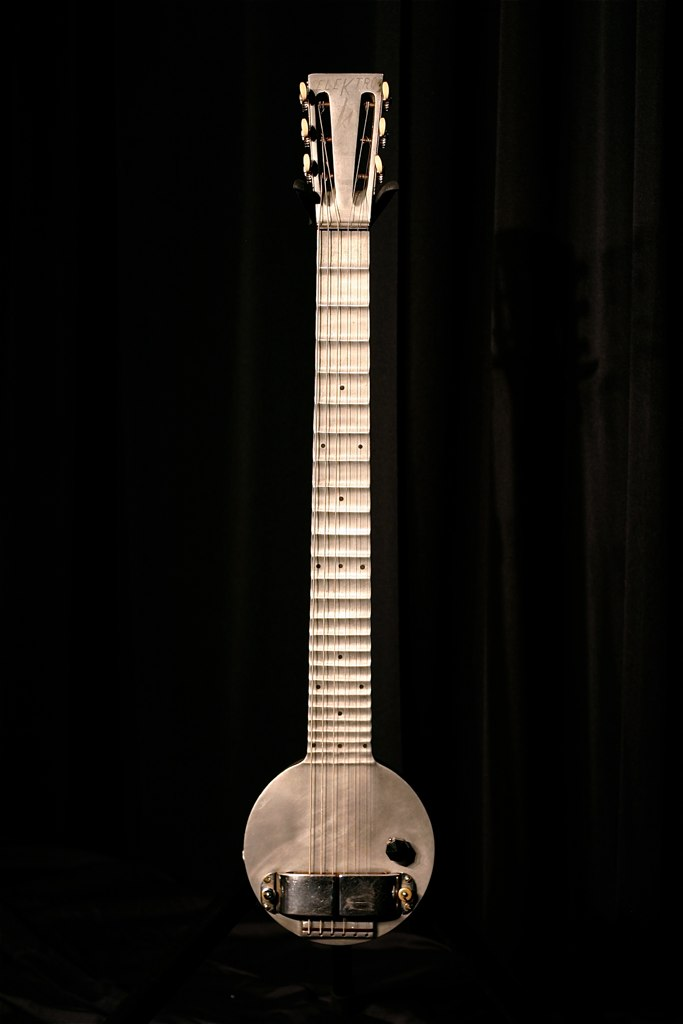
\includegraphics[width=.4\linewidth]{img/frying-pan}
	\caption{Beauchamp's ``Frying Pan'' (Museum of Making Music)}
	\label{fig:frying-pan}
\end{figure}

\paragraph*{}
The guitar pickup is unmistakably the most important piece of an electric
guitar. It is the device which translates the mechanical oscillatory motion of
the strings into an electrical signal vibrations of the strings. Today,
electric guitars and electric pickups come in various forms.

\subsubsection{Electric guitar pickup types}

\paragraph*{}
Electric guitar pickups are either passive or active. Active guitar pickups can
be thought of as passive guitar pickups with a preamp stage at the output of
the passive filter.

\paragraph*{}
Today, there are two widespread electric guitar pickup types: the
\textit{single-coil} electric guitar pickup and the \textit{humbucker}.

\paragraph*{}
The single-coil electric pickup was the one originally created by Beauchamp and
innovators of his time. It was relatively simple to create and manufacture and
was based on a simple physical phenomenon.

\paragraph*{}
With amplifiers becoming louder and more powerful, musicians noticed that their
single-coil pickups were picking up electromagnetic interference (due to their
antenna-like properties) as well as the motion of the strings. In 1955,
\textit{Seth Lover} invented the \textit{humbucher}. The humbucker promised to
solve this problem by combining two single-coil pickups which were connected in
reverse polarity, effectively canceling out the electromotive force generated
from external fields.

\paragraph*{}
This paper considers only single-coil pickups, as they are the most popular,
widespread and simple to use.

\subsubsection{Musical background}

\paragraph*{}
Musical instruments in general operate on musical scales. Musical scales are 
sets of ordered tones, ordered in ascending fundamental frequencies. The 
guitar's strings are $E$, $A$, $D$, $G$, $B$, $E$ whose frequencies are 
$82.41\si{Hz}$, $110.00\si{Hz}$, $146.83\si{Hz}$, $196.00\si{Hz}$, 
$246.94\si{Hz}$ and $329.63\si{Hz}$, respectively. It is worth noting that the 
relationship between the linear increase of tones and the respective frequency 
of the tone is exponential. This is due to the fact that human ears hear pitch 
in a logarithmical fashion, so it is necessary to compensate for this 
biological factor.

\subsubsection{Classical guitar operation}
\paragraph*{}
Although the classical guitar is not explored in this research paper, the basic
theory of its operation is necessary to understand the operation of the 
electric guitar. A model guitar is given in \ref{fig:ac-guitar}.
\begin{figure}[ht]
	\centering
	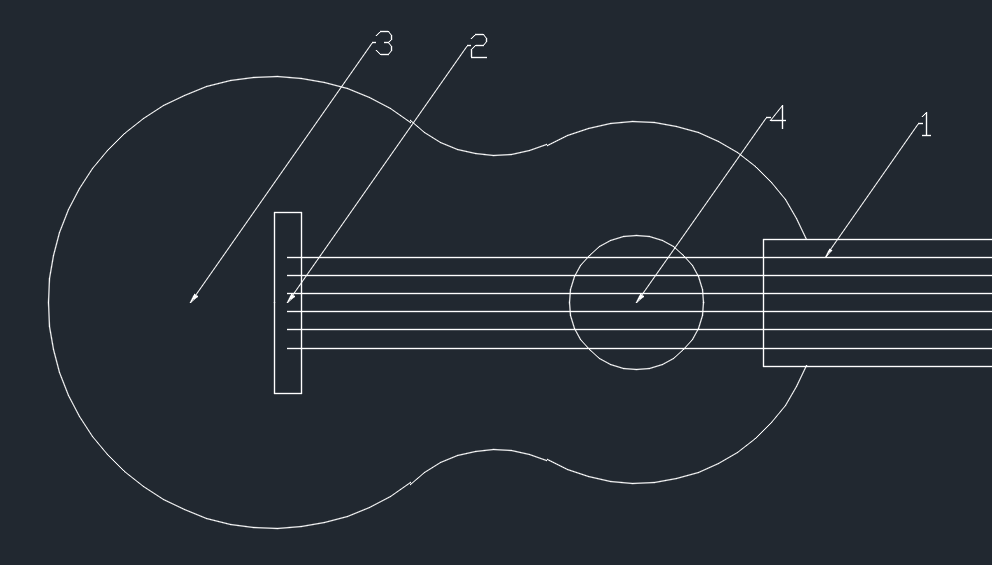
\includegraphics[width=.5\textwidth]{img/ac-guitar}
	\caption{A model of an acoustic guitar}
	\label{fig:ac-guitar}
\end{figure}
When the string $(1)$ is plucked, it resonates two main components of the 
guitar through the bridge $(2)$ - the top $(3)$\footnote{The ``top'' is the 
name given to the top wooden plate on the guitar.} and the air inside the 
cavity $(4)$, effectively creating \textit{Heimholtz resonance}
\footnote{Heimholtz resonance is a phenomenon of air resonating inside a body 
	with a cavity (Wolfe).}. The top resonates better with higher frequencies 
and the \textit{Heimholtz resonance} at play is better with lower frequencies.

\subsubsection{Electric guitar pickup operation}
\paragraph*{}
The electric guitar operates similarly to the acoustic guitar, except that 
instead of resonance playing the role of amplifying audio, a \textit{pickup} 
is used to pick the motion of the string up. The power outputted by the 
electric pickup is low, and is then amplified by an amplifier to be played on 
an electric speaker. An electric guitar pickup is given in figure 
\ref{fig:pickup}. 
\begin{figure}[ht]
	\centering
	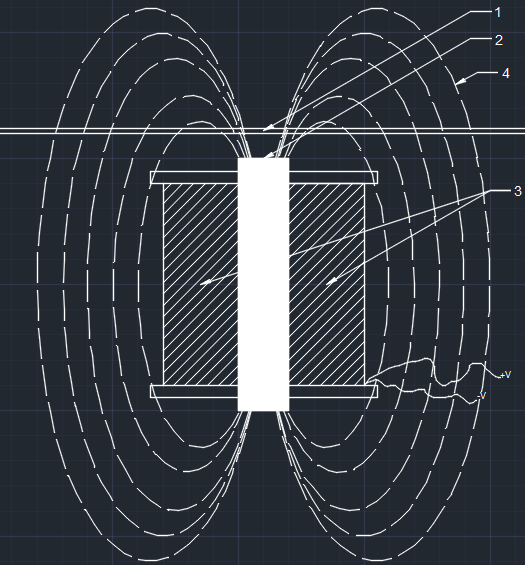
\includegraphics[width=.4\textwidth]{img/pickup}
	\caption{A model of an electric guitar pickup}
	\label{fig:pickup}
\end{figure}
When a string $(1)$ is strung on top of the permanently magnetized bobbin 
$(2)$, which is surrounded by very thin electrically insulated conducting wire 
$(3)$, it becomes magnetized. When the string is plucked, the surrounding 
magnetic field causes the magnetic field of the bobbin $(4)$ to be disturbed, 
causing the individual point charges in the wire $(3)$ to experience a 
\textit{Lorentz force}
\footnote{Lorentz force is the force that is exerted on a particle moving 
	through an electric and magnetic field (The Editors of Encyclopaedia 
Britannica).}. Because of this, an electromotive force appears in the wire 
$(3)$ which is linearly dependent on the motion of the string $(1)$.

\subsubsection{String harmonic series}
\paragraph*{} 
The string, as any oscillating body with fixed ends, creates harmonic series - 
sequences of sinusoidal tones whose frequencies are integer multiples of the 
lowest frequency, ie. the fundamental frequency. How high the amplitude of the 
individual harmonics is depends on a multitude of factors - the thickness of 
the string, the material of the string, how it is attached to the bridge, 
et cetera.

\paragraph*{} 
Because of these harmonic series an interesting effect comes to pass when an 
electric pickup is used. The string oscillating over a pickup at multiple 
harmonics is given in figure \ref{fig:pickup-harmonics}. 
\begin{figure}[ht]
	\centering
	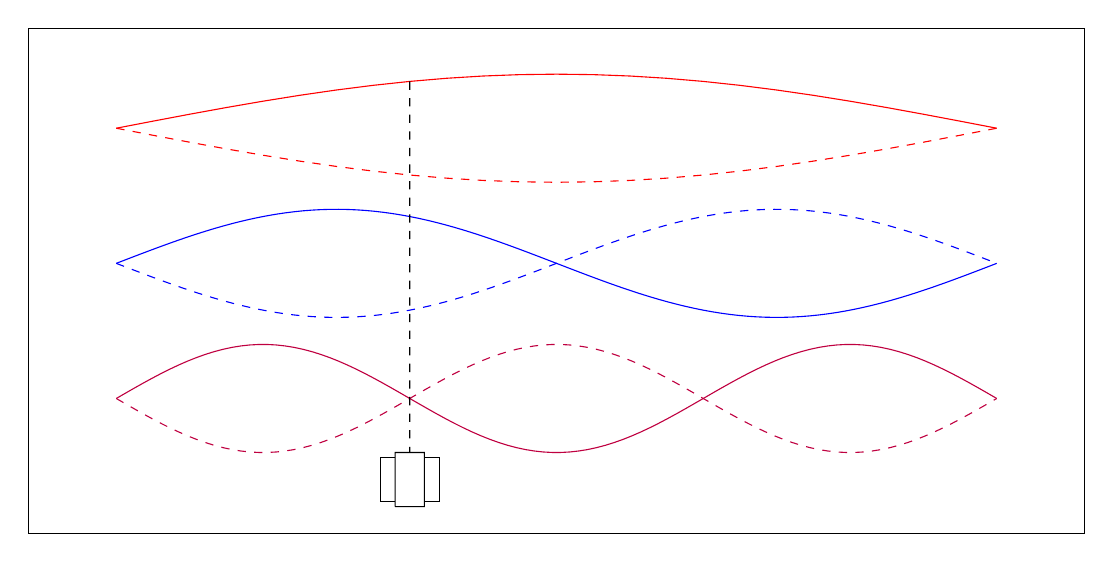
\begin{tikzpicture}
		\begin{axis}[
				ticks=none,
				width=15cm,
				height=8cm,
				ymin=-7.5
		]
			\addplot[
				color=red,
				domain=-1:1,
			]{abs(cos(deg(- pi * x * 0.5)))};
			\addplot[
				color=red,
				dashed,
				domain=-1:1
			]{-cos(deg(-pi*x*0.5))};
			\addplot[
				color=blue,
				domain=-1:1,
				samples=100
			]{-sin(deg(pi * x)) - 2.5};
			\addplot[
				color=blue,
				domain=-1:1,
				samples=100,
				dashed
			]{(sin(deg(pi * x))) - 2.5};
			\addplot[
				color=purple,
				domain=-1:1,
				samples=100
			]{sin(deg(1.5 * pi * x - pi/2)) - 5};
			\addplot[
				color=purple,
				domain=-1:1,
				samples=100,
				dashed
			]{-sin(deg(1.5*pi*x - pi/2)) - 5};
			\draw [>=stealth, dashed] (-0.33333333, 0.865) -- (-0.333333,-6);
			\draw (-0.3666666, -7) -- (-0.3, -7) -- (-0.3, -6) -- (-0.366666,
			-6) -- (-0.36666, -7); \draw (-0.3666666, -6.1) -- (-0.4, -6.1) --
			(-0.4, -6.9) -- (-0.366666, -6.9); \draw (-0.3, -6.1) --
			(-0.2666666, -6.1) -- (-0.2666666, -6.9) -- (-0.3, -6.9);
		\end{axis}
	\end{tikzpicture}
	\caption{The string oscillating over multiple harmonics over a pickup}
	\label{fig:pickup-harmonics}
\end{figure}
As is visible from the figure, at the position of the pickup, the string 
oscillates at the fundamental frequency and the second harmonic frequency, 
however, the third harmonic waveform is at the node at the position of the 
pickup, and therefore the harmonic is not picked up. Note also, that the 
pickup will not pick up the first or the second harmonic maximally, as at the 
line parallel to the magnet intersecting the string, the string is not at its 
anti-node.

\paragraph*{} 
A single harmonic can be modeled as a sine wave:
\begin{equation} 
	w(t) = A \sin ( 2 \pi n \nu_0 t),
	\label{eqn:basic-harmonic}
\end{equation}
where $A_m$ is the amplitude of the waveform, $n$ is the number of the 
harmonic from $n=1$ to $n=\infty$ and $\nu_0$ is the frequency of the 
fundamental harmonic.

\paragraph*{} 
Since the maximal amplitude at the location of the pickup will not be equal to 
the amplitude of the waveform itself, it is necessary to derive the formula 
for the amplitude of the waveform at the location of the pickup. This is 
achieved as follows.

\paragraph*{} 
Consider the waveform given in figure \ref{fig:harmonic-1-rel}.
\begin{figure}[ht]
	\centering
	\begin{tikzpicture}
		\begin{axis}[
				ymin=-1.7,
				ticks=none,
				width=15cm,
				height=6cm
		]
			\addplot[
				color=red,
				domain=-1:1,
			]{abs(cos(deg(- pi * x * 0.5)))};
			\draw [<->,>=stealth, dashed] (-1,-1.1) -- (-0.333333,-1.1);
			\draw [>=stealth, dashed] (-0.33333333, 0.865) -- (-0.333333,-1.15);
			\draw [<->,>=stealth, dashed] (-1,-1.4) -- (1,-1.4);
			\draw [>=stealth, dashed] (-1, 0) -- (-1,-1.45);
			\draw [>=stealth, dashed] (1, 0) -- (1,-1.45);
			\node at (0,-1.25) {$D$};
			\node at (-0.66666667,-0.95) {$d$};
		\end{axis}
	\end{tikzpicture}
	\caption{The relationship between the distance of the pickup from the 
	leftmost position and the amplitude at the pickup.}
	\label{fig:harmonic-1-rel}
\end{figure}
Because the shape of the string is sinusoidal, it follows that the 
relationship between the distance $d$ of the pickup from the leftmost position 
and the amplitude at the pickup is sinusoidal as well. 

\paragraph*{}
If one were to think of figure \ref{fig:harmonic-1-rel} as a function, it is 
the general function of:
$$f_A(x) = k_{h_1} \sin\Big(\frac{2\pi}{2 D} x\Big)$$
Note the use of the constant $k_h$. The constant $k_h$ is in place due to the 
fact that the amplitude of a harmonic depends heavily on the way the string is 
plucked, the sustain of the musical instrument, the string tension, and other 
effects. Usually the most powerful harmonic is the first one, although this is 
not a rule.

\paragraph*{}
It can be inferred that the amplitude $A$, when $d$ is substituted for $x$ is 
equal to:
\begin{equation}
	A = k_{h_1} \sin\Big(\pi \frac{d}{D}\Big)
	\label{eqn:harmonic-1-amp}
\end{equation}

\paragraph*{}
For the second harmonic, the graph is plotted in figure 
\ref{fig:harmonic-2-rel}.
\begin{figure}[ht]
	\centering
	\begin{tikzpicture}
		\begin{axis}[
				ymin=-1.7,
				ticks=none,
				width=15cm,
				height=6cm
		]
			\addplot[
				color=red,
				domain=0:1,
			]{sin(deg(pi * x * 2))};
			\draw [<->,>=stealth, dashed] (0,-1.1) -- (0.333333,-1.1);
			\draw [>=stealth, dashed] (0.3333333, 0.865) -- (0.333333,-1.15);
			\draw [<->,>=stealth, dashed] (0,-1.4) -- (1,-1.4);
			\draw [>=stealth, dashed] (0, 0) -- (0,-1.45);
			\draw [>=stealth, dashed] (1, 0) -- (1,-1.45);
			\node at (0.5,-1.25) {$D$};
			\node at (0.166666667,-0.95) {$d$};
		\end{axis}
	\end{tikzpicture}
	\caption{The relationship between the distance of the pickup from the 
	leftmost position and the amplitude at the pickup.}
	\label{fig:harmonic-2-rel}
\end{figure}

\paragraph*{}
One can infer from figure \ref{fig:harmonic-2-rel} that the value of amplitude 
$A$ is:
\begin{equation}
	A = k_{h_2} \sin\Big(2 \pi \frac{d}{D}\Big)
	\label{eqn:harmonic-2-amp}
\end{equation}

\paragraph*{}
It follows from equations \ref{eqn:harmonic-1-amp} and 
\ref{eqn:harmonic-2-amp} that the general formula is equal to:
\begin{equation}
	A_n = k_{h_n} \sin\Big(n \pi \frac{d}{D}\Big),
	\label{eqn:harmonic-general-amp}
\end{equation}
where $n$ is the number of the harmonic, $n = 1, 2, 3, 4\dots$

\paragraph*{}
When this derived amplitude is substituted into equation 
\ref{eqn:basic-harmonic}, the final formula is derived for a single harmonic:
\begin{equation}
	w(t) = k_{h_n} \sin\Big(n \pi \frac{d}{D}\Big) \sin(2 \pi n \nu_0 t)
	\label{eqn:general-harmonic}
\end{equation}

\paragraph*{}
To exemplify how the amplitude changes with increasing distance from the 
left-most position of the pickup, a graph is given in figure 
\ref{fig:harmonic-amp-relation}.

\begin{figure}[ht]
	\centering
	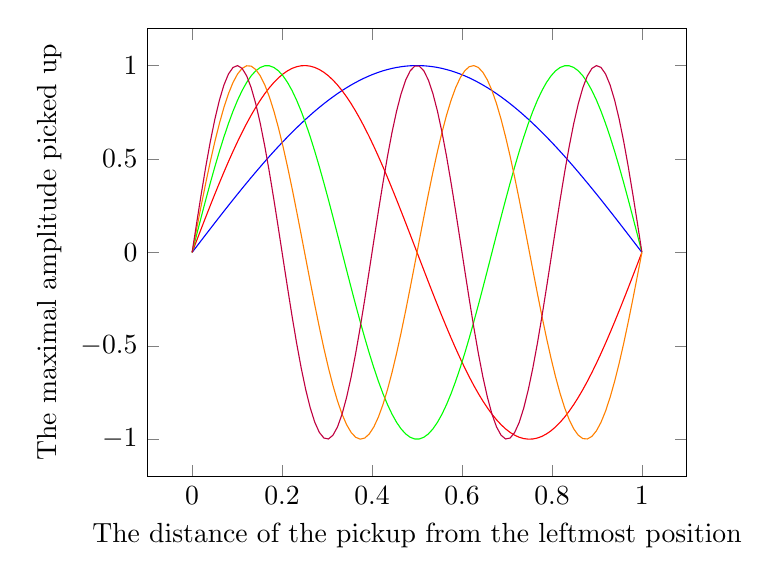
\begin{tikzpicture}
		\begin{axis}[
			xlabel=The distance of the pickup from the leftmost position,
			ylabel=The maximal amplitude picked up]
			\addplot[
				domain=0:1,
				samples=100,
				color=blue
			]{sin(deg(1 * pi * x / 1))};
			\addplot[
				domain=0:1,
				samples=100,
				color=red
			]{sin(deg(2 * pi * x / 1))};
			\addplot[
				domain=0:1,
				samples=100,
				color=green
			]{sin(deg(3 * pi * x / 1))};
			\addplot[
				domain=0:1,
				samples=100,
				color=orange
			]{sin(deg(4 * pi * x / 1))};
			\addplot[
				domain=0:1,
				samples=100,
				color=purple
			]{sin(deg(5 * pi * x / 1))};
		\end{axis}
	\end{tikzpicture}
	\caption{The relationship of the amplitude and the distance of the pickup 
	from the leftmost position for the first five harmonics in relative units}
	\label{fig:harmonic-amp-relation}
\end{figure}

\paragraph*{}
Given that the individual harmonic waves are superimposing, the final waveform 
will be a sum of all individual harmonics:
$$f(t) = \sum_{n=0}^{\infty} k_{h_n} \sin \bigg(n \pi \frac{d}{D} \bigg) 
\sin \bigg(2 \pi n \nu_0 t \bigg)$$
To differentiate these individual harmonics, it is necessary to find their 
amplitudes at different frequencies. The Fourier transformation is perfect for 
this goal.

\subsection{The Fourier transformation}

\subsubsection{Introduction}

\paragraph*{}
The Fourier transformation is a function which converts an input signal given
in the time domain to the frequency domain. In mathematical terms, for a
signal $S(t)$, it will create a function $\hat{S}(\nu)$ where $\nu$ represents
frequency.

\paragraph{} 
Suppose the graph of $S(t)$ is as given in figure \ref{fig:unk-func}.
\begin{figure}[ht]
	\centering
	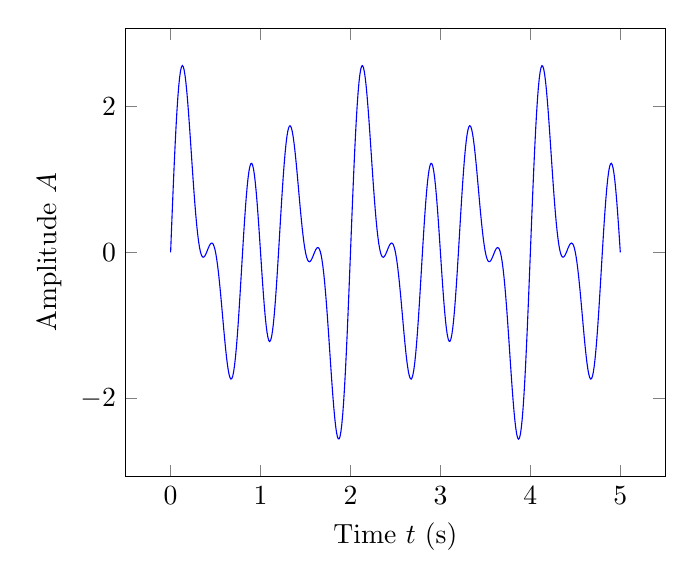
\begin{tikzpicture}
		\begin{axis}[
				xlabel=Time $t\text{ }(\si{s})$,
			ylabel=Amplitude $A$]
			\addplot[
				domain=0:5,
				samples=500,
				color=blue
			]{sin(deg(2 * pi * x)) + sin(deg(3 * pi * x)) + sin(deg(5 * pi *
			x))};
		\end{axis}
	\end{tikzpicture}
	\caption{The graph of an unknown signal $S(t)$}
	\label{fig:unk-func}
\end{figure}

\paragraph*{}
We shall suppose that $S(t)$ is a sum of sine and cosine waves. Now a question
is posed - how can we resolve the amplitudes and the frequencies of the
individual constituent sine and cosine waves?

\paragraph*{}
The Fourier transformation, in physical values (ie. time and frequency) is
defined as the following:
$$\hat{S}(\nu) = \int_{-\infty}^{\infty} S(t) e^{-2 \pi i t \nu} dt$$
Note the Fourier transformation is complex. Because of its complex domain, it
is used for both sine and cosine waves.

\paragraph*{}
The Fourier transformation creates a graph equal to the one given in figure
\ref{fig:ft-unk-func}\footnote{This is not an exact graph of the Fourier
	transformation of this function. Due to there being only three constituent
	sine waves, the computer algorithm that I've employed has created some
	inaccuracies. The derivative of a more accurate graph would not be as high
	as it is in the one I present, at the points of inflexion around the values
	of $2$, $3$ and $5$. However, for the purposes of exemplifying my point,
the graph is sufficiently accurate.}. Note how the graph shows peaks at values
$2$, $3$ and $5$ $\si{Hz}$. The graph is saying that the individual constituent
frequencies were precisely that - $2\si{Hz}$, $3\si{Hz}$ and $5\si{Hz}$. The
original signal was therefore:
$$S(t) = \sin(2 \pi t) + \sin(3 \pi t) + \sin(5 \pi t)$$

\begin{figure}[ht]
	\centering
	\begin{tikzpicture}
		\begin{axis}[
				xlabel=Frequency $\nu\text{ }(\si{Hz})$,
				ylabel=Amplitude]
				\addplot table [mark=none, y=A, x=f]{Data/four-plot.dat};
		\end{axis}
	\end{tikzpicture}
	\caption{The Fourier transformation of $S(t)$, $\hat{S}(\nu)$}
	\label{fig:ft-unk-func}
\end{figure}

\subsubsection{Derivation}

\paragraph*{}
To prove the Fourier transformation, a definition of what the Fourier series is
is necessary.

\subsubsection{Fourier series}

\paragraph*{}
The Fourier series is a method of representing arbitrary periodic functions as 
a sum of simple sine and cosine functions. A method for deriving it follows.

\paragraph*{}
Suppose an even function such as the one graphed in figure 
\ref{fig:odd-arb-func} exists.
\begin{figure}[ht]
	\centering
	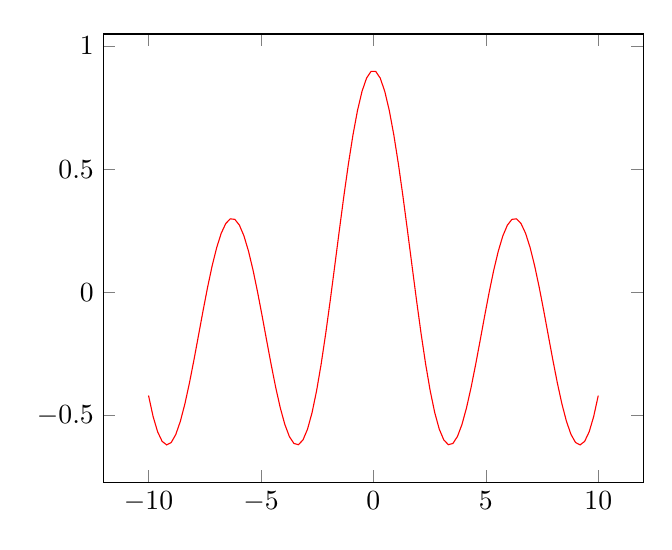
\begin{tikzpicture}
		\begin{axis}
			\addplot[
				color=red,
				domain=-10:10,
				samples=100
			]{0.3 * cos(deg(0.5 * x)) + 0.6 * cos(deg(x))};
		\end{axis}
	\end{tikzpicture}
	\caption{An arbitrary even function}
	\label{fig:odd-arb-func}
\end{figure}

The premise is that it is possible to express this function as a sum of cosine 
waves:
$$f(t) = \sum^{\infty}_{n=0}a_n \cos(2 \pi n t)$$

It is necessary to calculate the values of $a_n$. This problem is done in the 
following manner:

\paragraph*{}
Both sides are multiplied by $\cos(2 \pi m t)$:
$$f(t) \cos(2 \pi m t) = \sum^{\infty}_{n=0}b_n \cos(2 \pi n t) \cos(2 \pi m t)$$
Next, both sides are integrated over one period of the function, and the 
trigonometric identity of the product of cosines is employed:
\begin{equation}
	\begin{aligned}
		\int_{T} f(t) \cos(2 \pi m t) dt &= 
		\int_{T} \sum^{\infty}_{n=0} a_n \cos(2 \pi n t) \cos(2 \pi m t) dt \\
		&= \sum^{\infty}_{n=0} a_n \int_{T} \cos(2 \pi n t) \cos(2 \pi m t) dt \\
		&= \frac{1}{2} \sum^{\infty}_{n=0} a_n \int_{T} (\cos( (m + n) 2 \pi t) + \cos( (m - n) 2 \pi t)) dt \\
	\end{aligned}
	\label{eqn:fourier-series-1}
\end{equation}
Suppose $m \geq 0$ (this is possible to suppose because $m$ is arbitrary, and 
more importantly, it is physically impossible for frequency to be negative). 
From this it follows that $\cos( (m + n) 2 \pi t)$ has $m + n$ oscillations 
in a single period $T$, and consequently, $m + n$ oscillations in the 
integration interval. Since this is true, when this function is integrated, 
the result is $0$\footnote{The proof for this is trivial, however, it is 
published by a third party online and is available to the reader at the 
following link: \url{http://planetmath.org/integraloveraperiodinterval}.}. 
Equation \ref{eqn:fourier-series-1} is then simplified to:
\begin{equation}
	\begin{aligned}
		\int_{T} f(t) \cos(2 \pi m t) dt &=
		\frac{1}{2} \sum^{\infty}_{n=0} a_n \bigg(\int_{T} \cos( (m + n) 2 \pi t) dt + 
		\int_{T} \cos( (m - n) 2 \pi t) dt \bigg) \\
		&= \frac{1}{2} \sum^{\infty}_{n=0} a_n \int_{T} \cos( (m - n) 2 \pi t) dt
	\end{aligned}
	\label{eqn:fourier-series-2}
\end{equation}
Since the cosine function is even, in a single period $T$ (the integration 
interval - from $-\frac{T}{2}$ to $\frac{T}{2}$) the following is true:
$$\cos( (m - n) 2 \pi t) = \cos( (n - m) 2 \pi t)$$
When $m = n$:
$$\cos( (m - n) 2 \pi t) = \cos(0) = 1$$
From these statements, the following follows:
\[
	\int_{T} \cos( (m - n) 2 \pi t) = 
	\begin{cases}
		\int_{T} \cos ( (m -n) 2 \pi t) dt = 0 & \text{when } m \neq n \\
		\int_{T} 1 \cdot dt = T & \text{when } m = n
	\end{cases}
\]
It is key to note that:
$$\forall (0 < m < \infty, 0 < n < \infty \land m \neq n) \rightarrow
\int_{T} cos( (m - n) 2 \pi t) dt = 0$$
From this it follows that the whole summation in equation 
\ref{eqn:fourier-series-2} can be reduced to the case when $m = n$:
$$\int_T = f(t) \cos(m 2 \pi t) dt = \frac{1}{2} a_m T$$
To get $a_m$ is trivial:
\begin{equation*}
	a_m = \frac{2}{T} \int_T f(t) \cos(m 2 \pi t) dt
\end{equation*}
Finally, replacing $m$ with $n$ we get:
\begin{equation}
	a_n = \frac{2}{T} \int_T f(t) \cos(m 2 \pi t) dt
	\label{eqn:fourier-series-amp}
\end{equation}

However, the case of $m = 0$ is not considered. This case gives the $y$ axis 
offset $a_0$. Substituting with $m = 0$ in equation \ref{eqn:fourier-series-1}, 
we get:
$$
\begin{aligned}
\int_{T} f(t) \cos(2 \pi m t) dt &= 
\sum^{\infty}_{n=0} a_n \int_{T} \cos(2 \pi n t) \cos(2 \pi m t) dt \\ 
\int_T f(t) \cos(0) dt &= \sum^{\infty}_{n=0} a_n \int_T \cos(2 \pi n t) \cos(0) dt \\
\int_T f(t) dt &= \sum^{\infty}_{n=0} a_n \int_T \cos(2 \pi n t) dt \\
\int_T f(t) dt &= T a_0
\end{aligned}$$
This gives the final result for the $y$ axis offset:
\begin{equation}
	a_0 = \frac{1}{T} \int_T f(t) dt
	\label{eqn:fourier-series-yoffset}
\end{equation}
This result is coincidentally intuitively the average of all of the $y$ values 
of the points of the function in a single period.

Odd functions are represented in a similar manner:
$$f_o(t) = \sum^{\infty}_{n=1} b_n \sin(2 \pi n t)$$
The coefficients $b_n$ are, then:
$$b_n = \frac{2}{T}\int_T f_o(t) \sin(2 \pi n t) dt$$
As the derivation is quite similar to the one for the even function, it has 
been omitted.

Since any arbitrary function $f(t)$ can be represented as a sum of odd and even 
functions:
$$f_o(t) = \frac{1}{2}(f(t) - f(-t))$$
$$f_e(t) = \frac{1}{2}(f(t) + f(-t))$$
$$f(t) = f_o(t) + f_e(t)$$
The Fourier series' components can be applied:
$$f(t) = a_0 + \sum^{\infty}_{n=1} (a_n \cos(2 \pi n t) + b_n \sin(2 \pi n t))$$
with the coefficients being:
$$a_0 = \frac{1}{T} \int_T f(t) dt$$
$$a_n = \frac{2}{T} \int_T f(t) \cos(2 \pi n t) dt, n \neq 0$$
$$b_n = \frac{2}{T} \int_T f(t) \sin(2 \pi n t) dt$$

It is possible to express the Fourier series in its complex form, using 
Euler's formulas:
$$cos \phi = \frac{e^{i\phi} + e^{-i\phi}}{2}$$
$$sin \phi = \frac{e^{i\phi} - e^{-i\phi}}{2i}$$
\begin{equation*}
	\begin{aligned}
		f(t) &=
		a_0 + \sum^{\infty}_{n=1}(a_n \cos(2 \pi n t) + b_n \sin(2 \pi n t)) \\
		& = a_0 + \sum^{\infty}_{n=1}\Big(
		a_n \frac{e^{i 2 \pi n t} + e^{-i 2 \pi n t}}{2} + 
		b_n \frac{e^{i 2 \pi n t} - e^{-i 2 \pi n t}}{2i}\Big) \\
		&= a_0 + \sum^{\infty}_{n=1} \frac{a_n - ib_n}{2}e^{2 \pi n t} +
		\sum^{\infty}_{n=1} \frac{a_n + ib_n}{2} e^{-2 \pi n t}
	\end{aligned}
\end{equation*}

Let us now define $c_n$ as 
$$c_n = \frac{a_n - i b_n}{2}$$

This gives the complex Fourier series:
\begin{equation*}
	f(t) = \sum^{\infty}_{n = - \infty} c_n e^{i 2 \pi t}
\end{equation*}
This is referred to as the \textit{synthesis} equation.

From this it follows that $c_n$, the complex Fourier coefficient, is:
\begin{equation*}
	\begin{aligned}
		c_n &= 
		\frac{1}{2} \cdot \bigg( \frac{2}{T} \int_T f(t) \cos(2 \pi n t) dt - 
		i \frac{2}{T} \int_T f(t) \sin(2 \pi n t) dt \bigg) \\
		&= \frac{1}{T} \int_T f(t) \cos(2 \pi n t) - i f(t) \sin(2 \pi n t) dt \\
		&= \frac{1}{T} \int_T f(t) \bigg( 
			\frac{e^{i 2 \pi n t} + e^{-i 2 \pi n t}}{2} - 
		i \frac{e^{i 2 \pi n t} - e^{-i 2 \pi n t}}{2i} \bigg) \\
		&= \frac{1}{T} \int_T f(t) \frac{2 e^{i 2 \pi n t}}{2} dt \\
		c_n &= \frac{1}{T} \int_T f(t) e^{-i 2 \pi n t} dt
	\end{aligned}
\end{equation*}
This is referred to as the \textit{analysis} equation. This equation gives 
spectral lines for a frequency $n$. Note that it is not continuous.

\subsubsection{The Fourier transformation derivation}

\paragraph*{}
The Fourier transformation can be thought of as a continuous version of the 
Fourier series:
$$\hat{f} (t) = \int^{\infty}_{-\infty} f(t) e^{-i 2 \pi \nu t} dt$$

\paragraph*{}
Let the Fourier transformation be defined as the limit of the analysis 
formula of the Fourier series as $T$ approaches infinity:
$$\hat{f} (t) = \lim_{T \rightarrow \infty} c_n = \lim_{T \rightarrow \infty} 
\int_{-T / 2}^{T / 2} f(t) e^{-i 2 \pi n t} dt$$
Note the factor $\frac{1}{T}$ is completely ignored, due to the fact that 
$\lim_{n \rightarrow \infty} \frac{1}{n} = 0$, which would ruin the function. 
This is far more relevant when doing the inverse Fourier transformation, 
however the inverse Fourier transformation is outside of the scope of this 
paper and therefore is not explored. The limit makes the spectral lines come 
closer, creating the final equation:
$$\hat{f} (t) = \int_{-\infty}^{\infty} f(t) e^{-i 2 \pi \nu t} dt$$
The power of this equation lies in the fact that it gives a continuous 
function showing the frequencies of a \textit{non-periodic} signal. In turn, 
it has practical applications in converting a signal from the time domain to 
the frequency domain.

\section{Method}

\paragraph*{}
When a Fourier transformation is ran on a waveform it produces a continuous 
function of frequency, showing precisely amplitudes of frequencies. To explore 
the relationship between the pickup position and the harmonic effects, it is 
necessary to look at a three-dimensional graph where one axis is the 
independent variable - the position of the pickup, and two dependent 
variables - the frequency and the amplitude.

\paragraph*{}
To measure the effect of pickup position on harmonics of the electric guitar, 
an electric guitar with a movable pickup was constructed, as shown in 
\ref{fig:custom-guitar}.
\begin{figure}[ht]
	\centering
	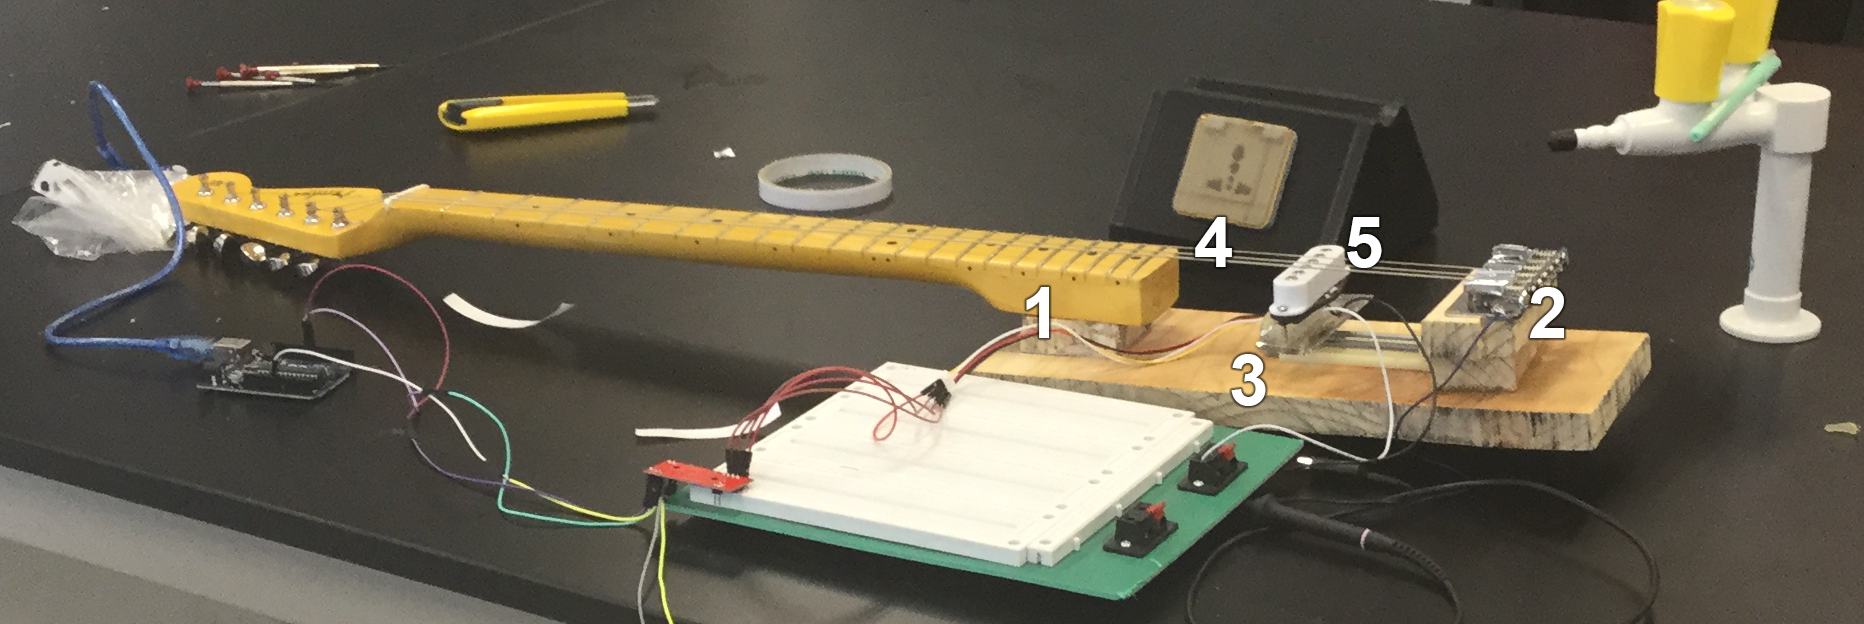
\includegraphics[width=.8\textwidth]{img/constructed-guitar}
	\caption{The constructed experimental electric guitar}
	\label{fig:custom-guitar}
\end{figure}
It has several major elements to it, similar to the normal electric guitar: 
(1) the neck of the electric guitar, (2) the bridge of the guitar, (3) the 
body of the guitar, (4) the strings, and, most notably, (5) a pickup whose 
position can be changed.

\paragraph*{}
The body of the guitar (3) was marked with hatch marks so the pickup could be 
set to a desired value. These hatch marks were marked using a ruler. They are 
shown in figure \ref{fig:hatch-marks}.
\begin{figure}[ht]
	\centering
	\includegraphics[width=.8\textwidth]{img/tally-marks}
	\caption{The hatch marks of the pickup position}
	\label{fig:hatch-marks}
\end{figure}
Since it was mechanically impossible to position the pickup immediately next 
to the bridge, the distance of the starting (left-most) position of the pickup 
was measured with a caliper.

\paragraph*{}
The pickup wires were connected to a \textit{GW Instek GDS-1000A-U} 
oscilloscope. The ground wire was also connected to the bridge of the electric 
guitar and the ground of the oscilloscope, to remove any potential noise that 
might occur\footnote{Due to being done in a building, there was a high chance
	that the strings would pick up the mains hum, so grounding them was
necessary.}, as given in figure \ref{fig:connection-schematic}.
\begin{figure}[ht]
	\centering
	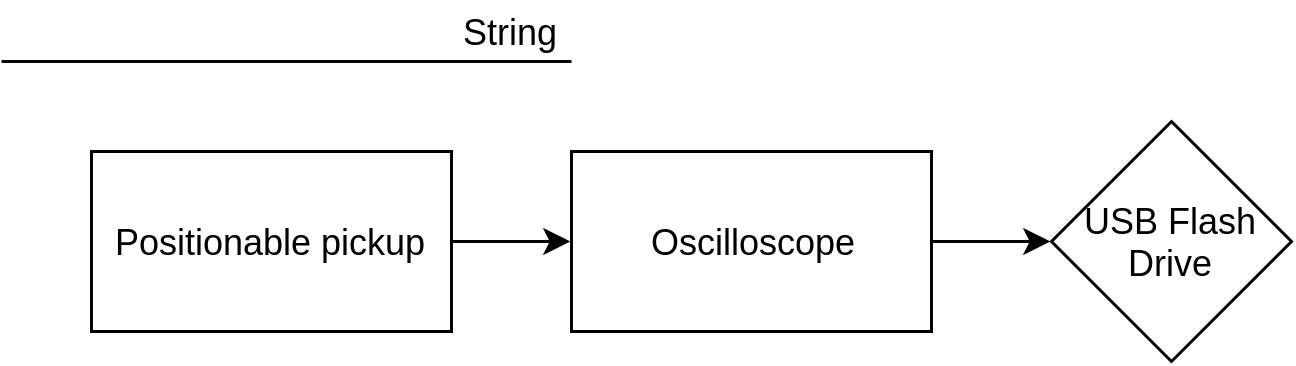
\includegraphics[width=.5\textwidth]{img/connection-schematic}
	\caption{A schematic of how the individual devices were connected}
	\label{fig:connection-schematic}
\end{figure}

\paragraph*{}
The string (4) was plucked for every position of the pickup. At the same time, 
the oscilloscope was set to record the waveform. The waveform was recorded 
using the oscilloscope and stored on a computer for further data processing. 
Measurements were done for all full-tones, until the first octave, of the 
guitar for the \textit{E} and \textit{A} strings.

\section{Data}

\subsection{Raw data}
\paragraph*{}
The recorded data was a collection of wave-forms in the \textit{CSV}\footnote{
Comma separated values} format, as the oscilloscope generated these files. As 
an example, the waveform for the \textit{E} string on the $5^{\text{rd}}$ fret 
is given in figure \ref{fig:wave-0-5-e} in the left-most pickup position.
\begin{figure}[ht]
	\centering
	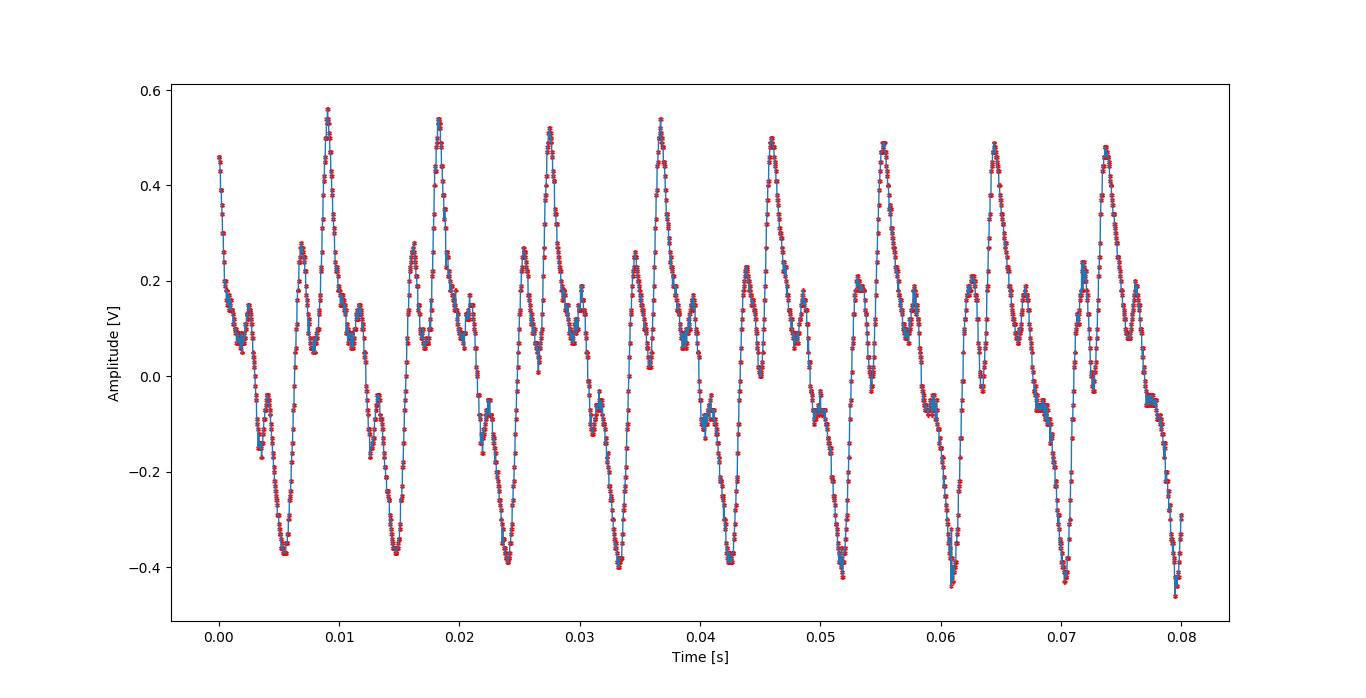
\includegraphics[width=\textwidth]{img/wave-0-5-e}
	\caption{The waveform of the \textit{E} string played on the 
	$5^{\text{rd}}$ fret in the left-most pickup position}
	\label{fig:wave-0-5-e}
\end{figure}

\paragraph*{}
Due to the fact that there has been a huge amount of data, it has been 
published online and is available at the following link: 
\url{
	https://github.com/markovejnovic/relationship-pickup-distance/tree/master/src/Data
}
A fraction of the available data is given in the appendix.

\paragraph*{}
The uncertainty for the \textit{GW Instek GDS-1000A-U} is $\pm 2 \si{mV}$ 
(Good Will Instrument Co., LTD).

\paragraph*{}
The left-most position of the pickup is not at a true $0$. The minimum offset 
of the pickup from the bridge could not be mechanically made to be $0$, and 
has been achieved to be equal to
$$d_0 = (31.6 \pm 0.01) \si{mm}$$
Note the very low value of the uncertainty. This has been achieved by using a 
caliper to measure $d_0$ from the bridge of the guitar.

\paragraph*{}
The uncertainty for the distance of the pickup from the left-most position $d$ 
can be calculated as follows. Since the hatch marks were copied from a ruler, 
the uncertainty during the copying is equal to $0.5\si{mm}$. Since the pickup 
was positioned at the copied hatch marks, the uncertainty increases by another 
$0.5\si{mm}$. Finally, the uncertainty increased when the distance from the 
bridge to the first hatch mark was measured with a caliper by the uncertainty 
of the caliper - $0.01\si{mm}$. The final uncertainty of $d$ is then:
$$\Delta d = \pm (0.5 + 0.5 + 0.01) \si{mm} = \pm 1.01 \si{mm}$$

\subsection{Data processing}

\paragraph*{}
The data processing was done in the \textit{python} programming language 
(Van Rossum, and L. Drake), \textit{numpy} (E. Oliphant) and 
\textit{matplotlib} (Hunter) as follows.

\paragraph*{}
First the oscilloscope data was loaded into memory, denoted here as a vector 
$w$, with the number of elements being $4000$. Next, the Fourier 
transformation was calculated of the waveform, showing the harmonics of the 
guitar:
$$f = \text{fft}(w)$$
Only the positive side of the Fourier transformation was used, due to 
the fact that the Fourier transformation in this case is symmetrical, as 
exemplified in figure \ref{fig:fou-0-5-e}.
\begin{figure}[ht]
	\centering
	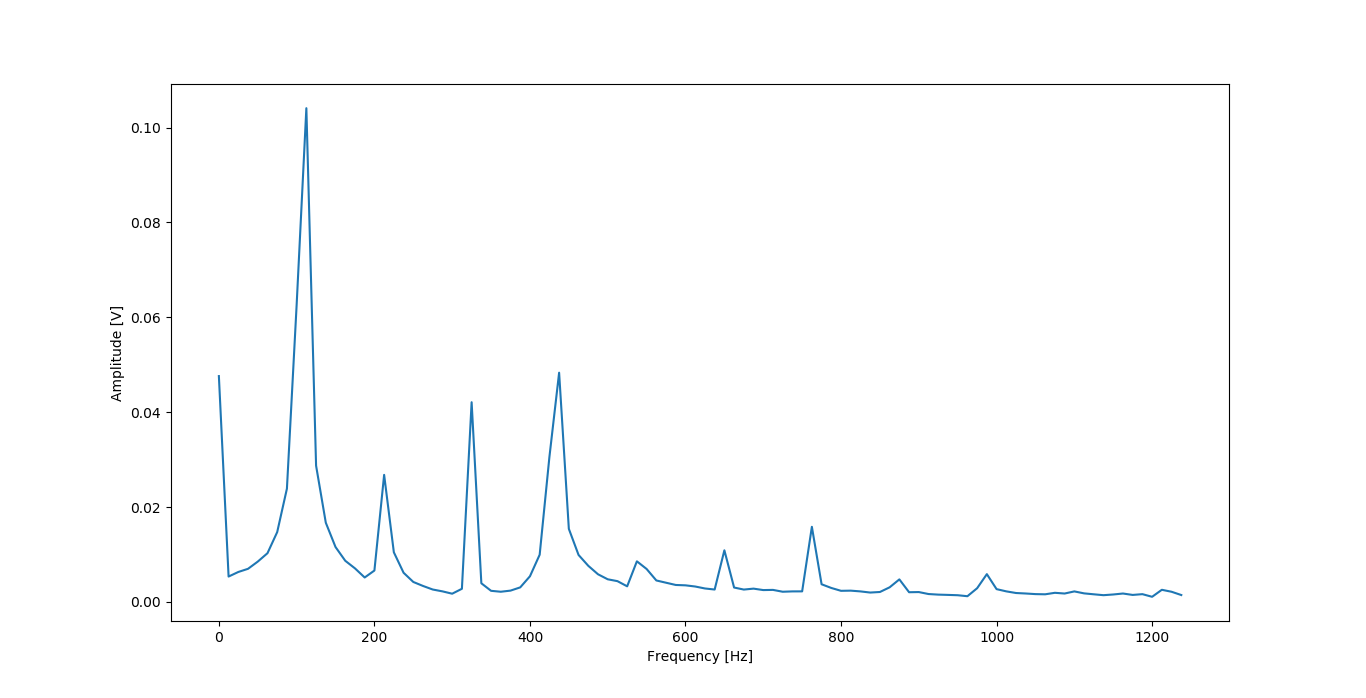
\includegraphics[width=\textwidth]{img/fou-0-5-e}
	\caption{The Fourier transformation of the played $5^{\text{th}}$ fret of 
	the \textit{E} string at the left-most pickup position}
	\label{fig:fou-0-5-e}
\end{figure}

\paragraph*{}
Next, the Fourier transformation was normalized, ie. mapped from $0$ to $1$ by 
multiplying the reciprocal of the highest scalar in the vector by the vector 
itself:
$$f' = \frac{1}{\max_{1 \leq i \leq N} w_i} \cdot f'$$
The previous example in figure \ref{fig:fou-0-5-e} becomes normalized as given 
in figure \ref{fig:fou-n-0-5-e}.
\begin{figure}[ht]
	\centering
	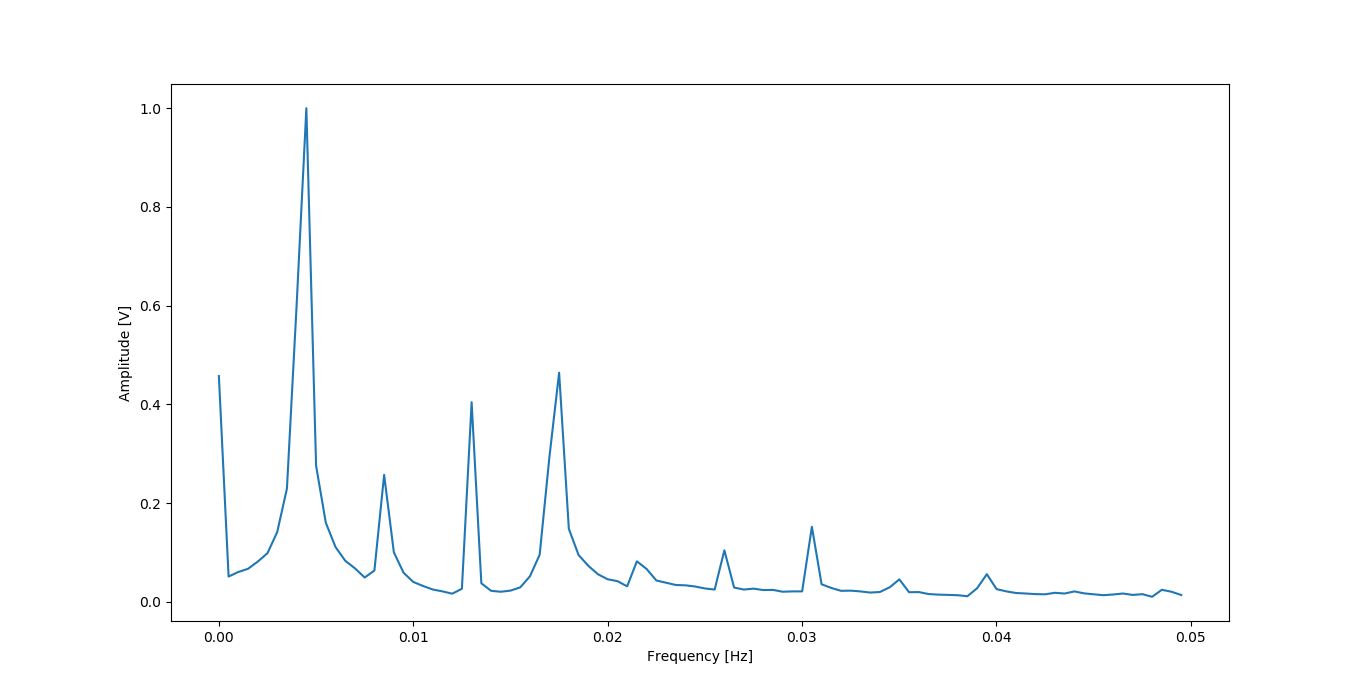
\includegraphics[width=\textwidth]{img/fou-n-0-5-e}
	\caption{The normalized Fourier transformation of the played 
		$5^{\text{th}}$ fret of the \textit{E} string at the left-most-pickup 
	position.}
	\label{fig:fou-n-0-5-e}
\end{figure}

\paragraph*{}
Once this has been done, the data was plotted on a three-dimensional graph 
where one axis was the independent pickup position, and the other two axes 
were dependent frequencies and amplitudes, as shown in figure 
\ref{fig:final-graph-u}.
\begin{figure}[ht]
	\centering
	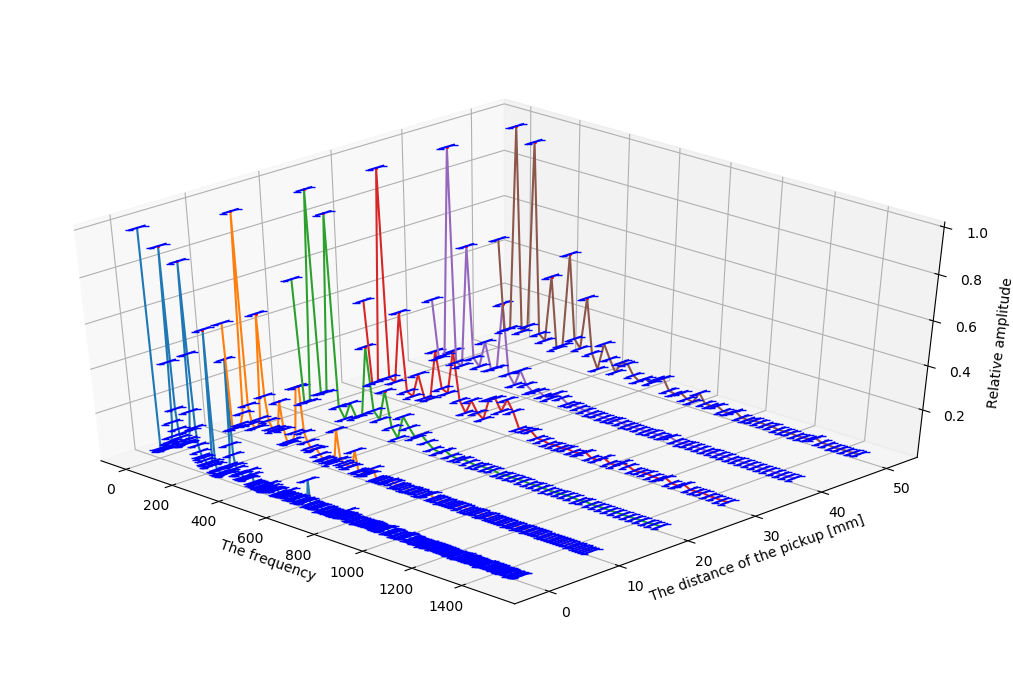
\includegraphics[width=\textwidth]{img/graph-final-u}
	\caption{The graph of the dependency of the frequency and amplitudes 
	with respect to the pickup position}
	\label{fig:final-graph-u}
\end{figure}

\paragraph*{}
Again, the sheer amount of data obstructs the ease of processing, so in figure 
\ref{fig:final-graph}, uncertainties have been omitted. Also, using the 
open-source algorithm \textit{peakutils} (Negri), Fourier peaks have been 
identified.
\begin{figure}[ht]
	\centering
	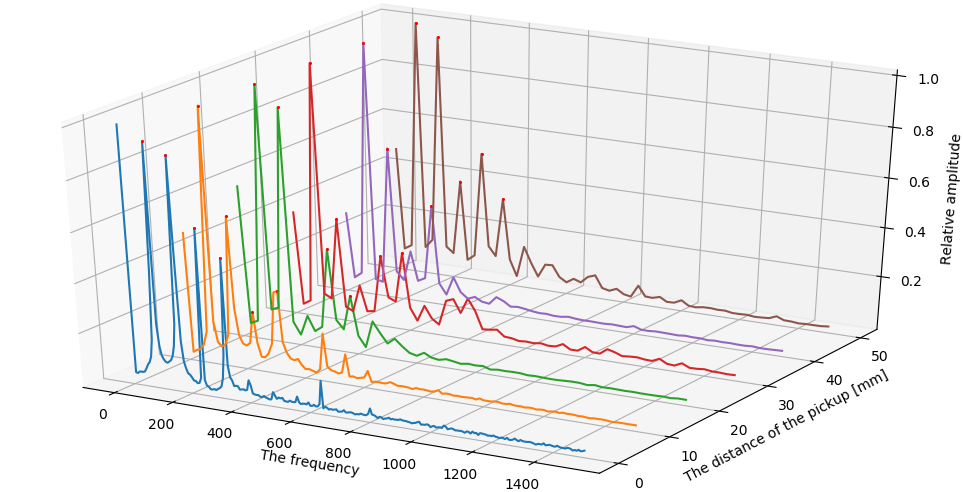
\includegraphics[width=\textwidth]{img/final-graph}
	\caption{The graph of the dependency of the frequency and amplitudes with 
	respect to the pickup position with omitted uncertainties and with 
identified Fourier peaks.}
	\label{fig:final-graph}
\end{figure}
Note that the first harmonics were completely omitted from identification. 
This is due to the fact that the Fourier transformation was somewhat 
incomplete, due to the waveform recorded by the oscilloscope being temporally 
very short, making the fundamental frequencies cut off, and therefore 
imprecise.

\paragraph*{}
Figure \ref{fig:final-graph-c} shows the same graph as figure 
\ref{fig:final-graph} with the peaks of the harmonics of different pickup 
positions being connected. This allows to follow how exactly, the pickup 
position moves.

\paragraph*{}
The code used to process the data is available both online at 
\url{https://github.com/markovejnovic/relationship-pickup-distance/tree/master/src} 
and in the appendix.

\begin{figure}[ht]
	\centering
	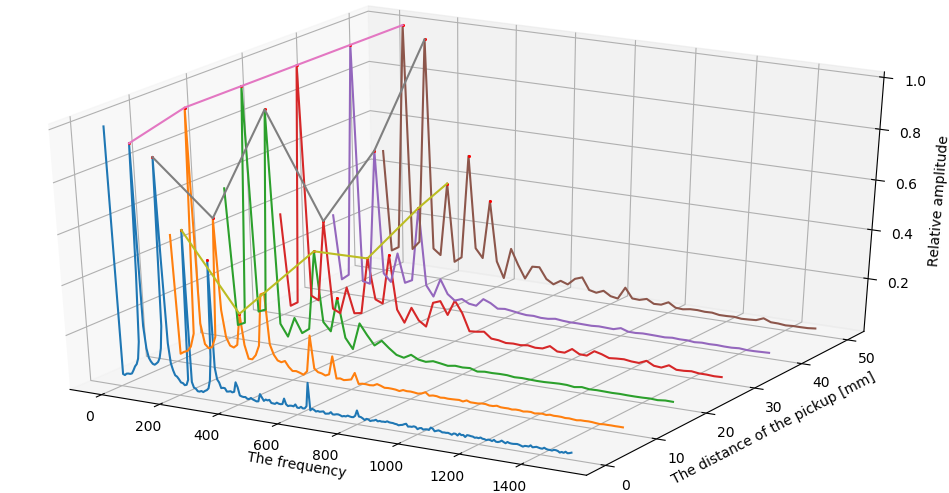
\includegraphics[width=\textwidth]{img/final-graph-c}
	\caption{The graph of the relationship of the harmonic amplitudes and the 
	pickup position with connected peaks.}
	\label{fig:final-graph-c}
\end{figure}

\section{Analysis}

\paragraph*{}
Considering that the scale length\footnote{The distance from the nut to the 
bridge of the guitar} of the \textit{Fender Stratocaster} is $648\si{mm}$ 
(``Scale Length Explained''), and the model guitar used in this experiment was 
constructed according to the \textit{Stratocaster} specification the distance 
from the nut to the bridge is equal to:
$$D = (648 \pm 0.5)\si{mm}$$

\paragraph*{}
From this and formula \ref{eqn:harmonic-general-amp} it follows that the
general formula of the relationship between the harmonic amplitude and pickup
position is:
$$\sin \bigg(n \pi \frac{d}{(648 \pm 0.5) \si{mm}} \bigg)$$

\paragraph*{}
In figure \ref{fig:final-graph-e}, the plot for the relationship between the
first $3$ harmonics and the position of the pickup $A(n, d)$ is given, as well
as the expected values calculated using the aforementioned formula.
\begin{figure}[ht]
	\centering
	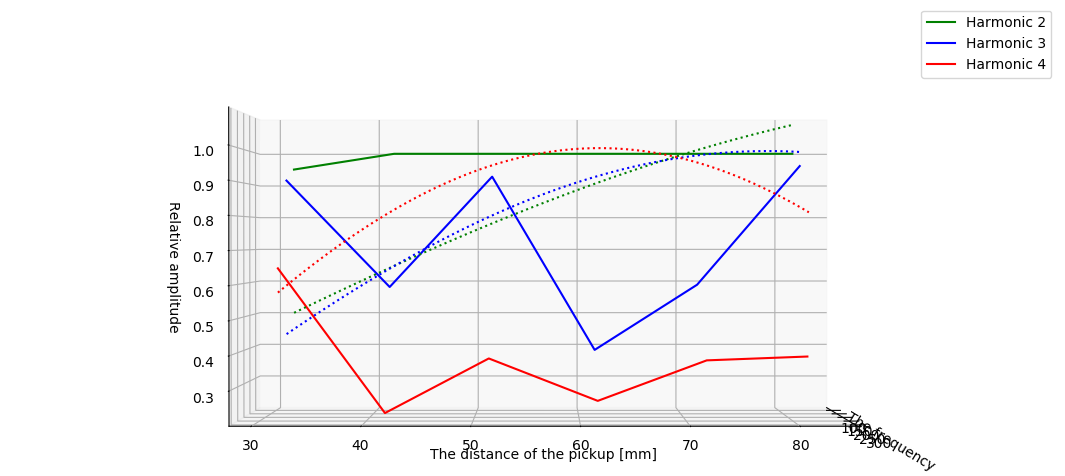
\includegraphics[width=\textwidth]{img/final-graph-e}
	\caption{The relationship between the amplitudes of the second, third and 
		fourth harmonics and the position of the pickup with the expected values}
	\label{fig:final-graph-e}
\end{figure}

\section{Evaluation}

\paragraph*{}
It is obvious that the measured relationship and the expected relationship are
widely apart. Although a minor part of the incorrectness can be attributed to
random error, it is implausible to classify such a high error to random error
alone.

\paragraph*{}
It is most certainly true that there were enormous systematic errors at play.
Two major possible sources of error, as well as other minor systematic errors
have been identified in the following sections.

\subsection{Poor harmonic identification}

\paragraph*{}
When the same graph as given in figure \ref{fig:final-graph-e} is observed 
from a top-down perspective, as given in figure \ref{fig:final-graph-e-t}, it 
becomes obvious that the peaks of the Fourier transformation are not colinear. 
\begin{figure}[ht]
	\centering
	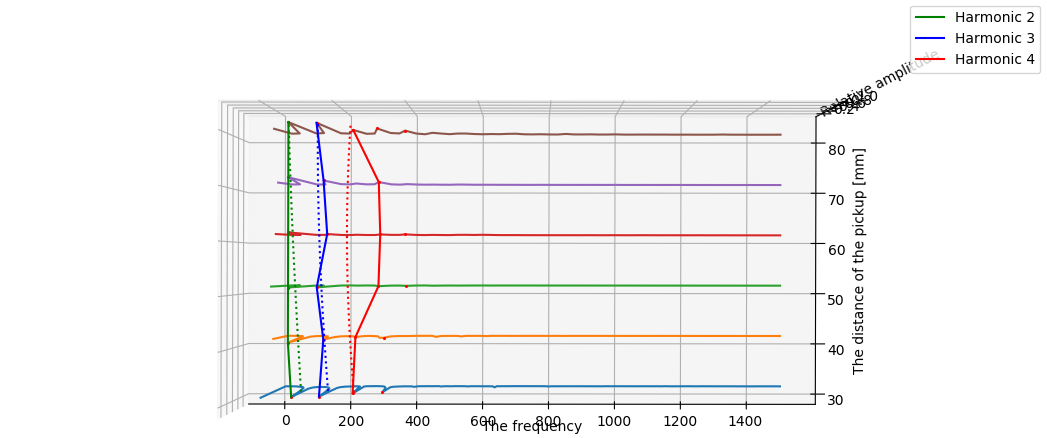
\includegraphics[width=\textwidth]{img/final-graph-e-t}
	\caption{The relationship between the amplitudes of the second, third and 
	fourth harmonics and the position of the pickup with the expected values 
as seen from a top-down perspective}
	\label{fig:final-graph-e-t}
\end{figure}
It is notable that the harmonics were poorly aligned. This poor alignment may 
stem from the following factor.

\subsection{Sustain}

\paragraph*{}
A guitar string, when first plucked, oscillates at multiple harmonics of
varying amplitudes. However, the sustain\footnote{Sustain is the time it takes
for a musical note to become inaudible, ie. to decay.} of each individual
harmonics is not equal. Because of this, certain harmonics will
decay\footnote{Their amplitude will decrease to a 0.} faster than others. This
data heavily indicates that, during the experiment, the minor difference in
time of recording waveforms for each pickup position affected the final Fourier
transformation in a major manner.

\subsection{Other minor effects}

\paragraph*{}
Other effects which could have affected the final Fourier transformation of 
the guitar waveform are the way the string was plucked, as plucking the string 
in a different manner creates a different tone; the gradual detuning of the 
guitar in an environment of varying temperature and mechanical impacts near 
the guitar which could have caused the strings to vibrate.

\section{Conclusion}

\paragraph*{}
The experiment results are inconclusive. Non-experimental observations point to 
there being a significant change in the tone of the guitar with the change of 
the position of the pickup. Donald Tillman's experimental results reaffirm 
this observation (Donald Tillman). However, the research conducted in this 
paper was unsuccessful to the point of showing no notable correlation.

\subsection{Rectifying errors}

\paragraph*{}
In the following, I have described possible solutions to the issues faced in 
this research paper.

\subsubsection{Sustain}
\paragraph*{}
To rectify the issue that was created during sustain, it would be best to 
record a complete waveform - from the plucking of the string to the complete 
decay of any sound. This would also rectify the issue of poor harmonic 
identification.

\subsubsection{Timbre from picking}
\paragraph*{}
To rectify the various different timbres that were encountered with different 
picking styles, it is necessary to construct a mechanism which can pick a 
string with a constant force and angle. A solenoid presents itself as an 
ideal solution, however, it is important for the solenoid to be far away from 
the pickup, so as not to interfere with the magnetic field generated by the 
pickup.

\subsection*{}
\paragraph*{}
Although the data is highly inconclusive, the experiment remains a valid one. 
As Donald Tillman's data shows, there are indeed effects on harmonics with the 
position of pickups. As the pickups move from the left-most position, 
Tillman's data shows that the frequency response moves translatory to the 
lower pitches, as the hypothesis suggests.

\clearpage
\pagebreak

\section*{Works cited}
\begin{hangparas}{.25in}{1}
Autodesk. \textit{Autocad 2014}. Version 19.1, Autodesk, 2014.\\

Chicago Music Exchange. \textit{Fender Stratocaster Sunburst 1956}. \url{https://images.reverb.com/image/upload/s--iiQ3rVKI--/a_exif,c_limit,e_unsharp_mask:80,f_auto,fl_progressive,g_south,h_1600,q_80,w_1600/v1497644319/ax58jibpcrmys6id16hl.jpg}. Accessed 29 Aug 2018.\\

Donald Tillman, J. ``Response Effects Of Guitar Pickup Position And Width''. 
\textit{Till.Com}, 2002, \url{http://www.till.com/articles/PickupResponse/.} 
Accessed 31 Aug 2018.\\

E. Oliphant, Travis. \textit{A Guide To Numpy}. Trelgol Publishing, 2006.\\

``Early History Of Rickenbacker''. \textit{Rickenbacker.Com},
\url{http://www.rickenbacker.com/history_early.asp}. Accessed 15 Oct 2018. \\


Good Will Instrument Co., LTD. \textit{GDS-1000-U Specifications}. Good Will 
Instrument Co., LTD, 
\url{https://www.gwinstek.com/en-global/products/downloadSeriesSpec/192}. 
Accessed 28 Aug 2018.\\
Guitar Center. \textit{Fender Special Edition HH Maple Fingerboard Standard 
Telecaster Sea Foam Pearl}. \url{https://www.guitarcenter.com/Fender/Special-Edition-HH-Maple-Fingerboard-Standard-Telecaster.gc}. Accessed 29 Aug 2018.\\

Hunter, John D. ``Matplotlib: A 2D Graphics Environment''. \textit{Computing 
In Science \& Engineering}, vol 9, no. 3, 2007, pp. 90-95. \textit{Institute 
Of Electrical And Electronics Engineers (IEEE)}, 
\url{doi:10.1109/mcse.2007.55}. Accessed 31 Aug 2018.\\

Museum of Making Music. \textit{Ro-Pat-In Cast Aluminum Electric Hawaiian
``Frying Pan'' Guitar}. 2009,
\url{https://commons.wikimedia.org/wiki/File:Elektrofryingpan.jpg}. Accessed 15
Oct 2018. \\

Negri, Lucas. \textit{PeakUtils}. Version 1.2.0, 2018.\\

``Scale Length Explained''. \textit{Stewmac.Com}, 2018, 
\url{https://www.stewmac.com/How-To/Online_Resources/Learn_About_Guitar_and_Instrument_Fretting_and_Fretw/Scale_Length_Explained.html}. Accessed 31 Aug 2018.\\

The Editors of Encyclopaedia Britannica. ``Lorentz Force''. 
\textit{Encyclopædia Britannica}, 2017, 
\url{https://www.britannica.com/science/Lorentz-force}. Accessed 31 Aug 2018.\\

Van Rossum, Guido, and Fred L. Drake. \textit{Python 3 Reference Manual}. 
Paramount, CA, 2009, \url{https://dl.acm.org/citation.cfm?id=1593511}. 
Accessed 28 Aug 2018.\\

Wolfe, Joe. ``Helmholtz Resonance''. \textit{Newt.Phys.Unsw.Edu.Au}, 
\url{http://newt.phys.unsw.edu.au/jw/Helmholtz.html}. Accessed 31 Aug 2018.\\

\end{hangparas}
\pagebreak

\section*{Appendix}
\addcontentsline{toc}{section}{Appendix}
\begin{appendices}

	\subsection*{Data processing code}
	\lstinputlisting[
		language=Python,
		frame=single,
		title=waveform.py
	]{../src/waveform.py}
	\lstinputlisting[
		language=Python,
		frame=single,
		title=data\_reader.py
	]{../src/data_reader.py}
	\lstinputlisting[
		language=Python,
		frame=single,
		title=util.py
	]{../src/util.py}
	\lstinputlisting[
		language=Python,
		frame=single,
		title=boiler.py
	]{../src/boiler.py}
	\lstinputlisting[
		language=Python,
		frame=single,
		title=plot\_ft.py
	]{../src/plot_ft.py}
	\lstinputlisting[
		language=Python,
		frame=single,
		title=plot.py
	]{../src/plot.py}

	\subsection*{Raw data}
	\paragraph*{}
	The following table shows the amplitudes of the guitar signal at sample
	times of 6 different pickup positions as outputted by the oscilloscope. The
	data shown here is for the $A$ string played at the $5^{\text{th}}$ fret.
	\csvreader[
		longtable=rrrrrrr,
		table head={
			\multirow{2}{*}{Sample time $t$ ($s$)} &
			\multicolumn{6}{c}{Voltage at position $d$ $[\times 5 \cdot 10^{-2}
			V]$} \\ \cline{2-7}
			& $0mm$ & $10mm$ & $20mm$ & $30mm$ & $40mm$ & $50mm$ \\ \hline \hline
		},
		late after line=\\\hline,
	]{Data/rawdata.csv}
	{t = \t, a = \a, b = \b, c = \c, d = \d, e = \e, f = \f}
	{\t & \a & \b & \c & \d & \e & \f}

\end{appendices}

\end{document}
